% !TEX root = Prokect199.tex
\subsection{Simplicial Complex}
    \begin{definition*}
    A $\textbf{simplicial complex} ~~\mathcal T$ in $\mathbb{R}^n$ is a finite set of simplices in $\mathbb{R}^n$ that satisfies the following conditions:
    \begin{enumerate}[label =\arabic*.]
      \item Any face of a simplex from $\mathcal{T}$ is also in $\mathcal{T}$.
      \item The intersection of any two simplices ${T}_1, {T}_2 \in \mathcal{T}$ is a face of both ${T}_1$ and  ${T}_2$.
    \end{enumerate}
    \begin{figure}[b]
    \centering
    %\includegraphics[width=60mm]{Figures/SimplicialComplex.png}
    \includegraphics[width=60mm]{SimplicialComplex}
    \caption[Simplicial Complex Example and Counterexample]{Adopted from~\cite{WEBSITE:1}}%cite???
    \label{Fig2}
    \end{figure}
    \end{definition*}
    In other words, the first condition asks $\mathcal{T}$ to be closed under subsimplices, and the second condition asks that the intersection of any two simplices is either a common subsimplex or empty because the empty set is a face of every simplex. Examples in 2D are shown in Figure.1. \\
    \indent
    Any subset ${T\textprime}\in{T}$ that is itself a simplicial complex is called a $\textit{subcomplex}$ of ${T}$. A $\textit{simplicial k-complex} ~~\mathcal T$ is a simplicial complex where the largest dimension of any simplex in $\mathcal T$ is ${k}$. So a simplicial 2-complex must not contain tetrahedra or higher dimension simplices. The 0-complex of ${T}$ is called a $\textit{vertex set}$ of ${T}$. We can also think simplicial complex as a space with a triangulation, which is the division of a surface or a plane polygon into a set of 2-simplices. The constrains of triangulation will be discussed in ? section.\\

    \paragraph{Simplicial Complex under Affine Transformation}\mbox{}\\
    Extending further from simplex under affine transformation, now we know that simplicial complex is just a finite set of simplices. Therefore, we can define the Transformed Simplicial Complex $F(\mathcal{T})$ as follows
    \begin{equation*}
    F(\mathcal{T}) := \{F(T) \quad \vert \quad T\in \mathcal{T}\}
    \end{equation*}
    If $\mathcal{T}$ is consistent, then $F(\mathcal{T})$ is also consistent by inheriting this property from $\mathcal{T}$.

    \paragraph{Shape Measure of Simplicial Complex}\mbox{}\\
    We define shape measure of a simplex \(T \in\mathbb{R}^n$ as $\mu({{T}}) = \displaystyle \frac{\operatorname{diam}({T})^k}{\operatorname{vol^k}({T})}\). Now consider a simplicial complex $\mathcal{T}\in\mathbb{R}^n$, we define the geometric shape measure $\mu(\mathcal{T})$ as follows,
    \begin{equation*}
    \mu(\mathcal{T}) = \max_{T \in \mathcal{T}} \mu(T)
    \end{equation*}
    By definition, we see that the shape measure of a simplicial complex $\mathcal{T}$ is the supreme of the set of shape measures of all simplex $T\in\mathcal{T}$. If the largest shape measure of a simplex in this simplicial complex is bounded, then none of simplices in $\mathcal{T}$ is degenerate. In other words, if simplex $T_0 \in\mathcal{T}$ is non-degenerate, then simplicial complex $\mathcal{T}$ non-degenerate.
    [Correct?? Pf needed???]